\usetikzlibrary{shapes,arrows}
\tikzstyle{block} = [draw, fill=blue!20, rectangle, 
    minimum height=3em, minimum width=4em]
\tikzstyle{circle} = [draw, fill=blue!20, ellipse, 
    minimum height=2.5em, minimum width=2.5em]
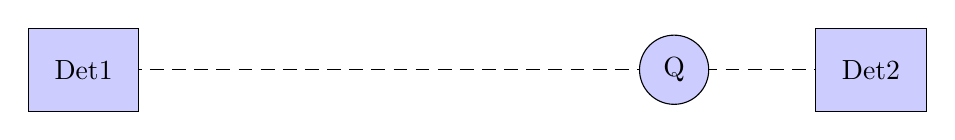
\begin{tikzpicture}
 \coordinate (L) at (-5,0);
 \coordinate (R) at (5,0);
\coordinate (A) at (2.5,4.3);
\coordinate (O) at (2.5,0);

\draw[dash pattern=on5pt off3pt] (L) -- (R);


\node[block, name=det1] at (L) {Det1};
\node[block, name=det2, rotate=0] at (R) {Det2};
\node[circle, name=source] at (O) {Q};

\end{tikzpicture}